\chapter{System Analysis}
\label{ch:system_analysis}

\section{Overview}
The \textbf{VR Driving Simulator} project aims to provide a high-fidelity training and evaluation environment for driving schools. 
The simulator models real-world driving dynamics using virtual reality and custom-built physical input devices (steering wheel, pedals, and gear shifter). 
This chapter outlines the system analysis, including its functional components, workflows, and overall system architecture.

\section{Objectives}
\begin{itemize}
    \item To design a modular VR-based driving simulation environment replicating realistic car control and behavior.
    \item To integrate Bluetooth-enabled hardware input devices for steering, acceleration, braking, and gear shifting.
    \item To ensure compatibility with the Meta Quest 3 headset (and optionally PC VR link) for immersive interaction.
    \item To provide performance analytics for driver evaluation and training improvement.
\end{itemize}

\section{System Components}
The proposed system consists of three major components:
\begin{enumerate} 
    \item \textbf{Hardware Interface:} The physical control setup — steering wheel, pedal set, and gear lever — connected via Bluetooth or USB.
    \item \textbf{Software Simulation:} Developed in Unity or Unreal Engine, containing vehicle physics, 3D environment, and UI.
    \item \textbf{VR Interface:} The Meta Quest 3 headset provides head tracking, stereoscopic rendering, and real-time feedback.
\end{enumerate}

\section{Model Diagram}
Figure~\ref{fig:model_diagram} illustrates the logical relationship between the hardware, software, and VR components.

\begin{figure}[H]
    \centering
    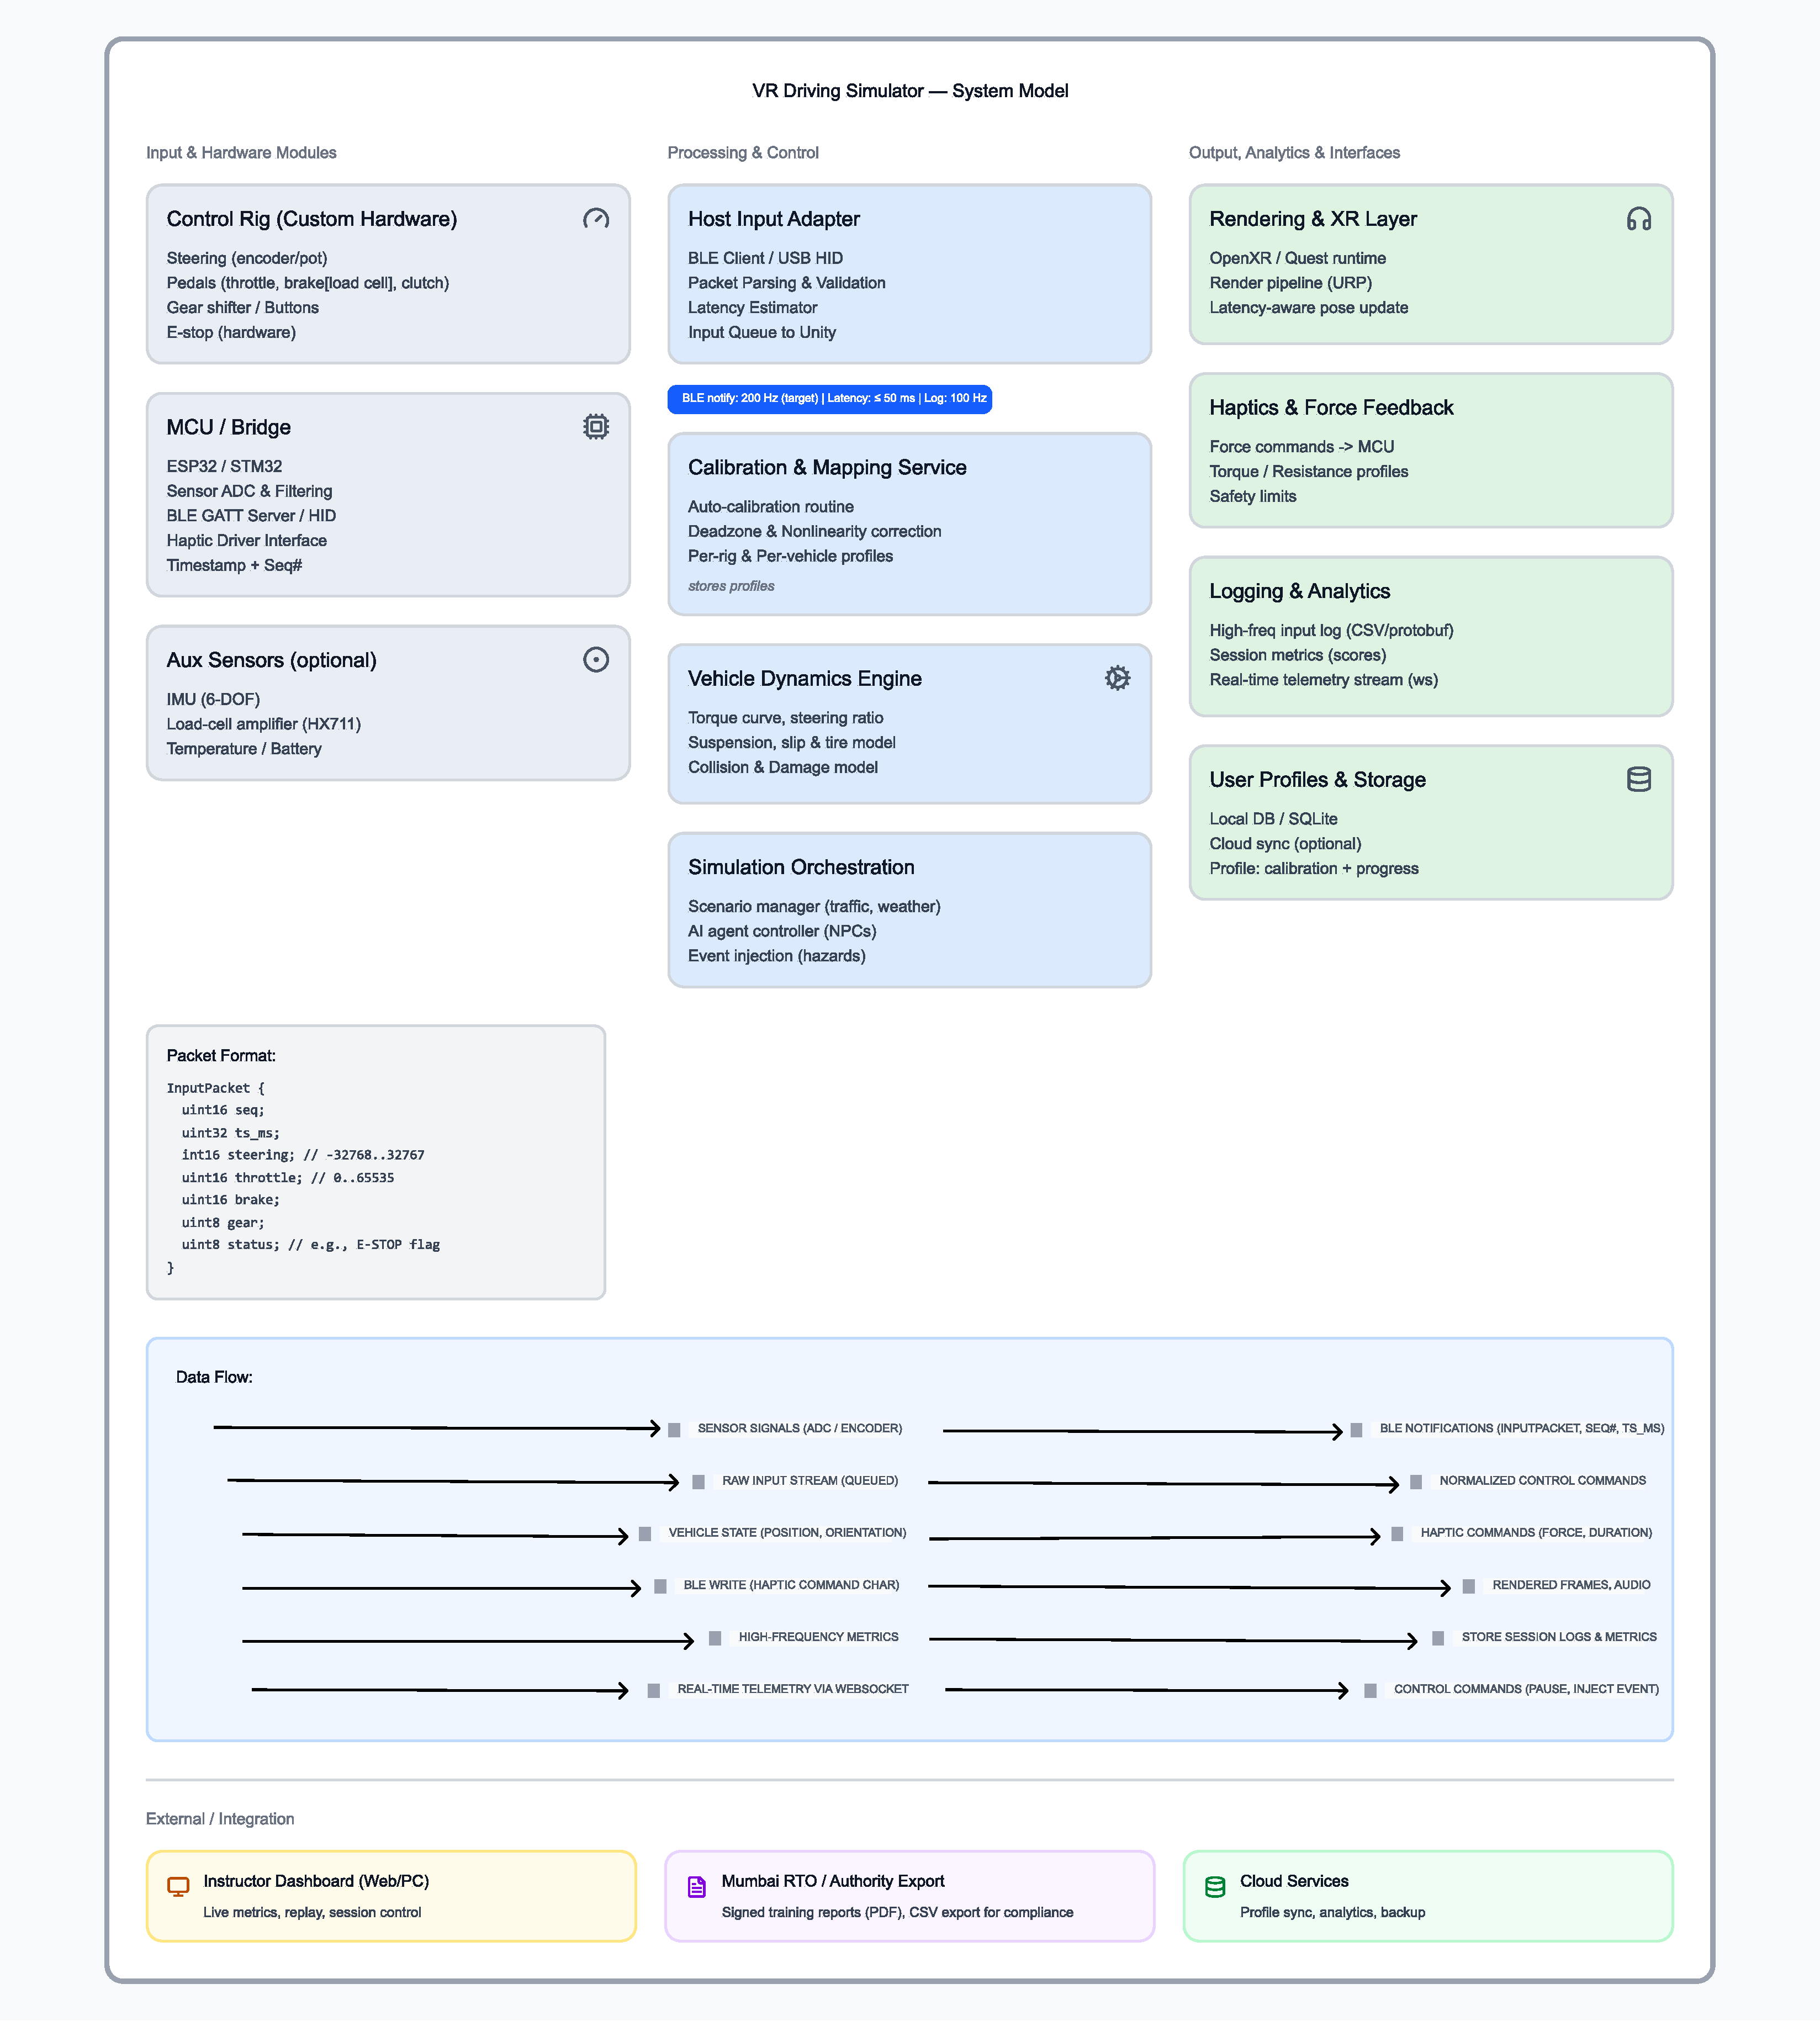
\includegraphics[width=0.9\textwidth]{figs/model_diagram.pdf}
    \caption{Model diagram of the proposed VR Driving Simulator system.}
    \label{fig:model_diagram}
\end{figure}

\section{System Architecture}
The system architecture describes how hardware inputs, simulation logic, and VR rendering interact.  
Data from the steering and pedal modules is transmitted to the main simulation engine, which processes it through a physics module and updates the rendered environment in real time.

\begin{figure}[H]
    \centering
    \includegraphics[width=0.95\textwidth]{figs/system_architecture.pdf}
    \caption{System architecture of the VR Driving Simulator.}
    \label{fig:system_architecture}
\end{figure}

\section{Workflow Diagram}
The workflow diagram (Figure~\ref{fig:workflow}) shows the sequential process of system operation — from initializing the simulation to user interaction and evaluation.

\begin{figure}[H]
    \centering
    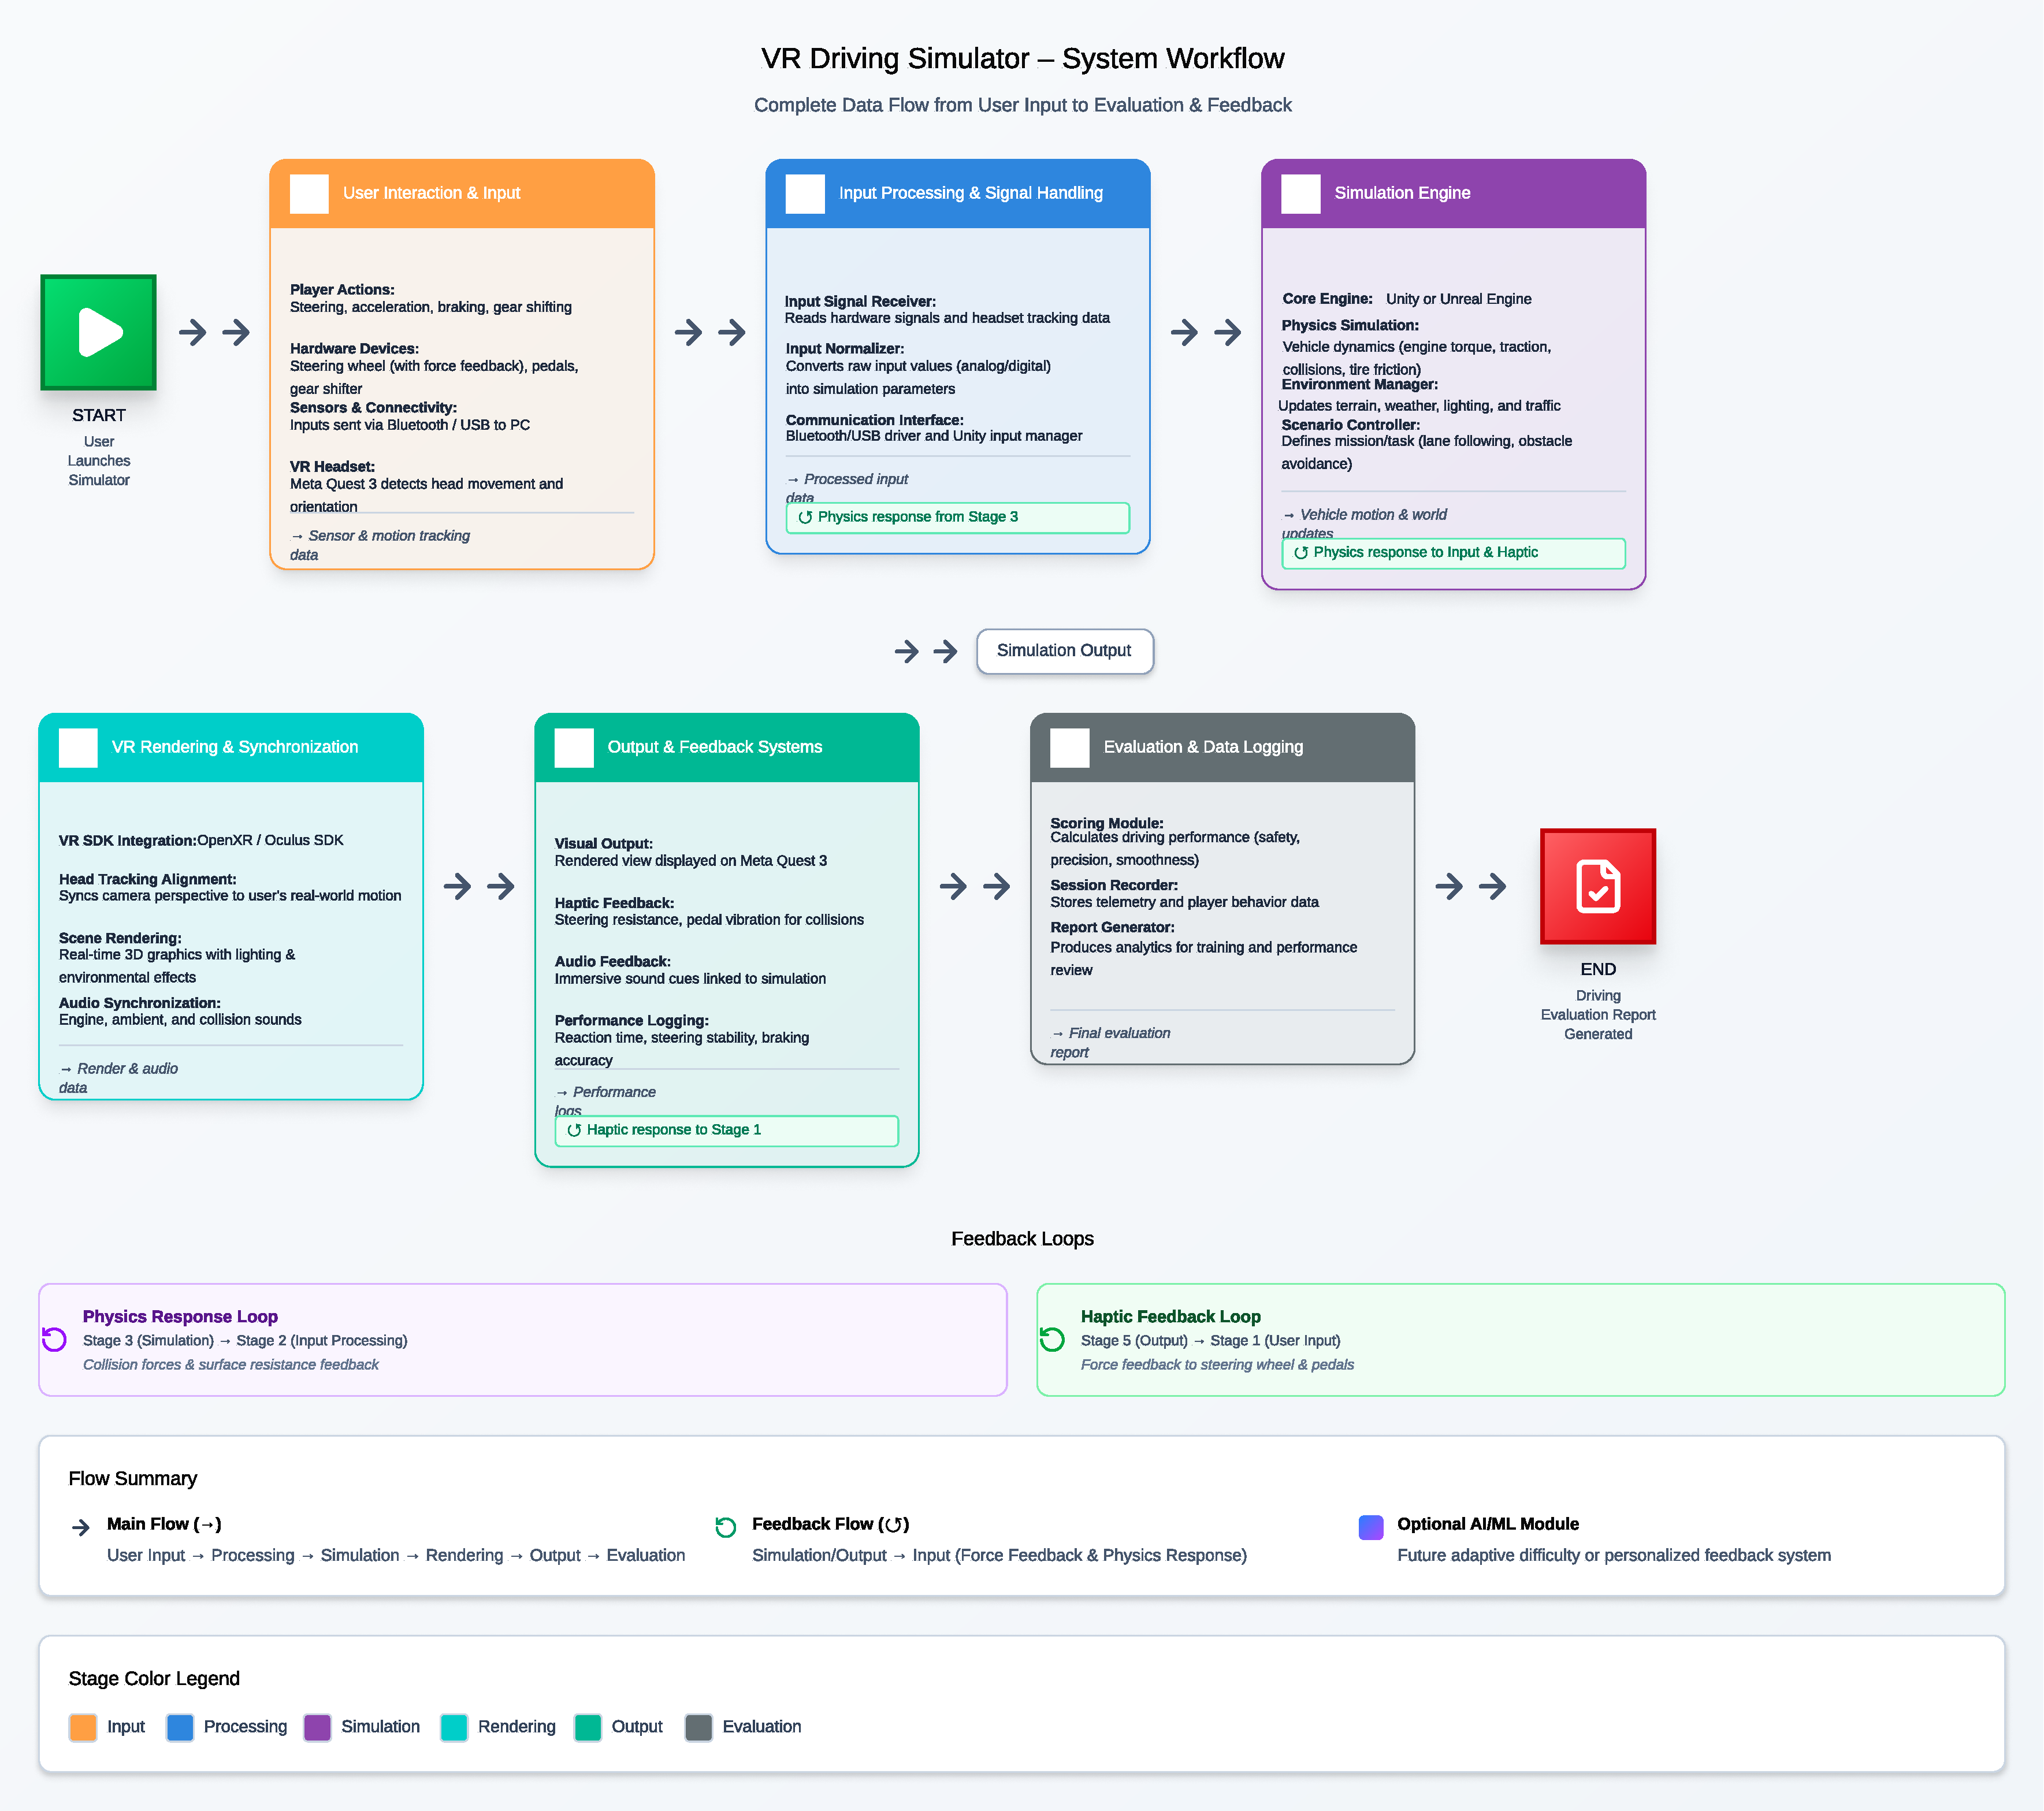
\includegraphics[width=0.9\textwidth]{figs/workflow_diagram.pdf}
    \caption{Workflow of the VR Driving Simulator system.}
    \label{fig:workflow}
\end{figure}

\section{Functional Flow}
\begin{enumerate}
    \item \textbf{Initialization:} Load vehicle and environment assets.
    \item \textbf{Hardware Connection:} Establish Bluetooth or USB input from the control devices.
    \item \textbf{Simulation Loop:} Capture input data, process physics, and update visuals.
    \item \textbf{VR Rendering:} Display stereo visuals through the Meta Quest 3 headset.
    \item \textbf{Performance Evaluation:} Record metrics such as braking efficiency, lane deviation, and speed consistency.
\end{enumerate}

\section{Conclusion}
This system analysis outlines how the proposed simulator integrates custom hardware, immersive VR visualization, and realistic physics. 
The subsequent chapter will focus on implementation and integration details.
